\documentclass{article}[]
\usepackage[utf8]{inputenc}
\usepackage{graphicx}
\usepackage{geometry}
\usepackage{float}
\usepackage{tabularx}
\usepackage[style=indexgroup]{glossaries}
\usepackage[table]{xcolor}
\usepackage{minted}
\usepackage{subcaption}
\usepackage{tikz}
\usepackage{multirow}
\definecolor{conv}{HTML}{E8E7EC}
\definecolor{pool}{HTML}{D7D8DA}
\definecolor{input}{HTML}{ffffff}
\definecolor{drop}{HTML}{F7F8FC}
\definecolor{dense}{HTML}{D5D6DA}
\definecolor{flat}{HTML}{F4F5FA}
\definecolor{output}{HTML}{B6B7B9}


\tikzset{conv/.style={black,draw=black,fill=conv,rectangle,minimum height=1cm}}
\tikzset{pool/.style={black,draw=black,fill=pool,rectangle,minimum height=1cm}}
\tikzset{input/.style={black,draw=black,fill=input,rectangle,minimum height=1cm}}
\tikzset{drop/.style={black,draw=black,fill=drop,rectangle,minimum height=1cm}}
\tikzset{dense/.style={black,draw=black,fill=dense,rectangle,minimum height=1cm}}
\tikzset{flat/.style={black,draw=black,fill=flat,rectangle,minimum height=1cm}}
\tikzset{output/.style={black,draw=black,fill=output,rectangle,minimum height=1cm}}


\setglossarystyle{super3colheaderborder}
\setlength{\glsdescwidth}{\linewidth}
\geometry{hmargin=2.5cm,vmargin=1.5cm}   
\pagenumbering{gobble}
\newglossaryentry{campagne}
{
    name=campagne,
    description={Processus qui englobe la collecte des données, l'analyse des résultats et l'évaluation des performances.}
} 


\newglossaryentry{GNSS}
{
name=GNSS,
description={Le Global Navigation Satellite System (GNSS) est un système de positionnement par satellite qui permet de déterminer avec précision la position d'un objet ou d'une personne sur la surface de la Terre.}
}

\newglossaryentry{RTK}
{
    name=RTK,
    description={Le Real Time Kinematic (RTK) est une technologie qui permet de corriger la position en temps réel, améliorant ainsi la précision des données de localisation .}
}

\newglossaryentry{crocodile}
{
    name=crocodile,
    description={Dans le contexte ferroviaire, le "crocodile" est un dispositif entre les rails qui transmet un signal en cabine à proximité d'un franchissement de signal et peut, si nécessaire, arrêter le train.}
}

\newglossaryentry{ETCS}
{
    name=ETCS,
    description={L'ETCS (European Train Control System) est un système automatique de sécurité ferroviaire européen qui prévient les dépassements de signaux rouges en transmettant des informations de signalisation et de vitesse aux conducteurs.}
}

\newglossaryentry{TensorFlow}
{
    name=TensorFlow,
    description={Librairie complète dédiée à la création et au déploiement simplifié de modèles de machine learning.}
}

\makeglossaries

\begin{document}
\thispagestyle{empty}
\begin{center}
    
\includegraphics[width=5cm]{images/umons.png}
    \hspace{90.0pt}
    
\includegraphics[width=5cm]{images/FS.png}	    
\end{center}
\vspace{4cm}	                               
\begin{center}	                              
    {\huge \bf Gestion Intelligente des Rails : Analyse du Ballast et Maintenance Prédictive}\\                        
    \vspace{3cm}
    \large Rapport réalisé dans le cadre du stage de  Master (en alternance) en Sciences Informatiques à Finalité Spécialisée Professionnelle (bloc 2) \\
    \vspace{1cm}
   Sous la direction de Stéphane Dupont\\
    \vspace{3cm}
    Faruk Oner  \\
    N° matricule 222423 \\

    \vfill	                                   
    Année académique 2023/2024
\end{center}

% \include{A) Font matter/2- Acknowledgements }
% \section*{\huge Avant-propos}
\vspace{2cm}
    \hfill\begin{minipage}{0.5\linewidth}
    % Ce rapport de stage décrit les activités réalisées et les résultats obtenus au cours de mon stage chez VINCI Energies Belgium. Ce stage a été effectué dans le but de développer et d'optimiser un système de gestion d'énergie (EMS), qui vise à optimiser la consommation énergétique d'un site, en équillibrant les différentes souces d'énergie, ainsi que les charges.\\
    
    % En tant que stagiaire,  mon principal objectif était de prédire les consommations futures en utilisant les séries temporelles existantes, et de préparer les données pour qu'elles soient utilisables par un algorithme de pilotage stratégique.\\

    % Bien que n'ayant aucune connaissance préalable dans les domaines des séries temporelles et de la data science, j'ai consacré un temps considérable à me former sur ces sujets au cours de mon stage. Cette expérience a été riche en enseignements et m'a permis d'acquérir une solide compréhension des principes et techniques impliquées dans ce domaine. \\

    % Ce rapport de stage décrit les défis auxquels j'ai été confronté, les solutions que j'ai trouvées et les résultats obtenus. Il montre également l'importance de l'apprentissage continu et de la détermination pour réussir dans un domaine nouveau et complexe. 
\end{minipage}


\newpage
\tableofcontents{\centering}
\clearpage % passe à la page suivante

\pagenumbering{arabic} 

\section{Introduction}
Ce stage s'inscrit dans le cadre de l'identification des paramètres fonctionnels (\textit{cf.} Section 1.3) visant à analyser le ballast afin de détecter les excès ou les manques de celui-ci. Cette introduction a pour objectif de présenter l'entreprise ainsi que le projet Hyperion (\textit{cf.} Section 1.2), grâce auquel le projet RHEA (\textit{cf.} Section 2) est né, en s'appuyant sur la documentation fournie par Cegelec \cite{Hyperion-interface}. Les objectifs que visa à atteindre ce projet sera également présenter.

\subsection{Présentation de l'Entreprise}

Vinci Energies Belgium est une filiale du groupe VINCI, un leader dans les secteurs de l'industrie, du tertiaire, des infrastructures et de l'ICT. Elle est engagée dans la transformation digitale et la transition énergétique à travers le déploiement de nouvelles technologies pour soutenir ses clients dans la réalisation de leurs projets. À travers ses 15 marques, elle offre des solutions allant de la conception à la réalisation, ainsi que des méthodes d'optimisation pour garantir la réussite de leurs projets. En tant que stagiaire, j'ai été recruté par la marque Cegelec Infra Technics, spécialisée dans l'ingénierie, le développement de logiciels et les technologies pour les projets d'infrastructure. Un contrat CIP (Convention d'Immersion Professionnelle) a été signé pour une durée de 8 mois, avec une charge horaire de 20 heures par semaine, dans le but de me permettre d'acquérir des compétences professionnelles hautement valorisantes. 

\subsection{Hyperion}

Cegelec Infra Technics en collaboration avec ADCIS, une compagnie spécialisée dans la vision par ordinateur et l'intelligence artificielle, a conçu le système Hyperion pour Infrabel dans le but de vérifier les données topographiques du réseau ferroviaire. Ce système utilise des capteurs de vision et de localisation installés sur deux trains de mesure, afin de recueillir des données précises sur l'infrastructure ferroviaire, permettant ainsi une comparaison avec les données réelles existantes. \\

\noindent Le système Hyperion est composé de deux composants.
\begin{itemize}
    \item Une unité d'acquisition embarqué dans le train (\textit{cf.} Figure 1) qui permet d'acquérir des données visuelles telles que les images, les profils du terrain, les nuages de points, ainsi que des données de navigation (\textit{cf.} Figure 2).
        \begin{figure}[H]
            \centering
            \fbox{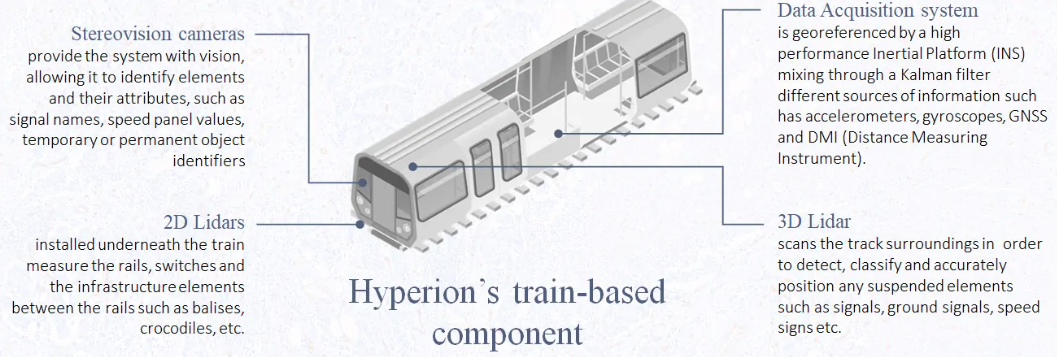
\includegraphics[width=15cm]{images/Hyperion-train-based-system.png}  } 
            \caption{Unité d'acquisition embarquée - ADCIS \cite{Hyperion-Unité}} 
        \end{figure}
        \begin{figure}[H]
            \centering
            \fbox{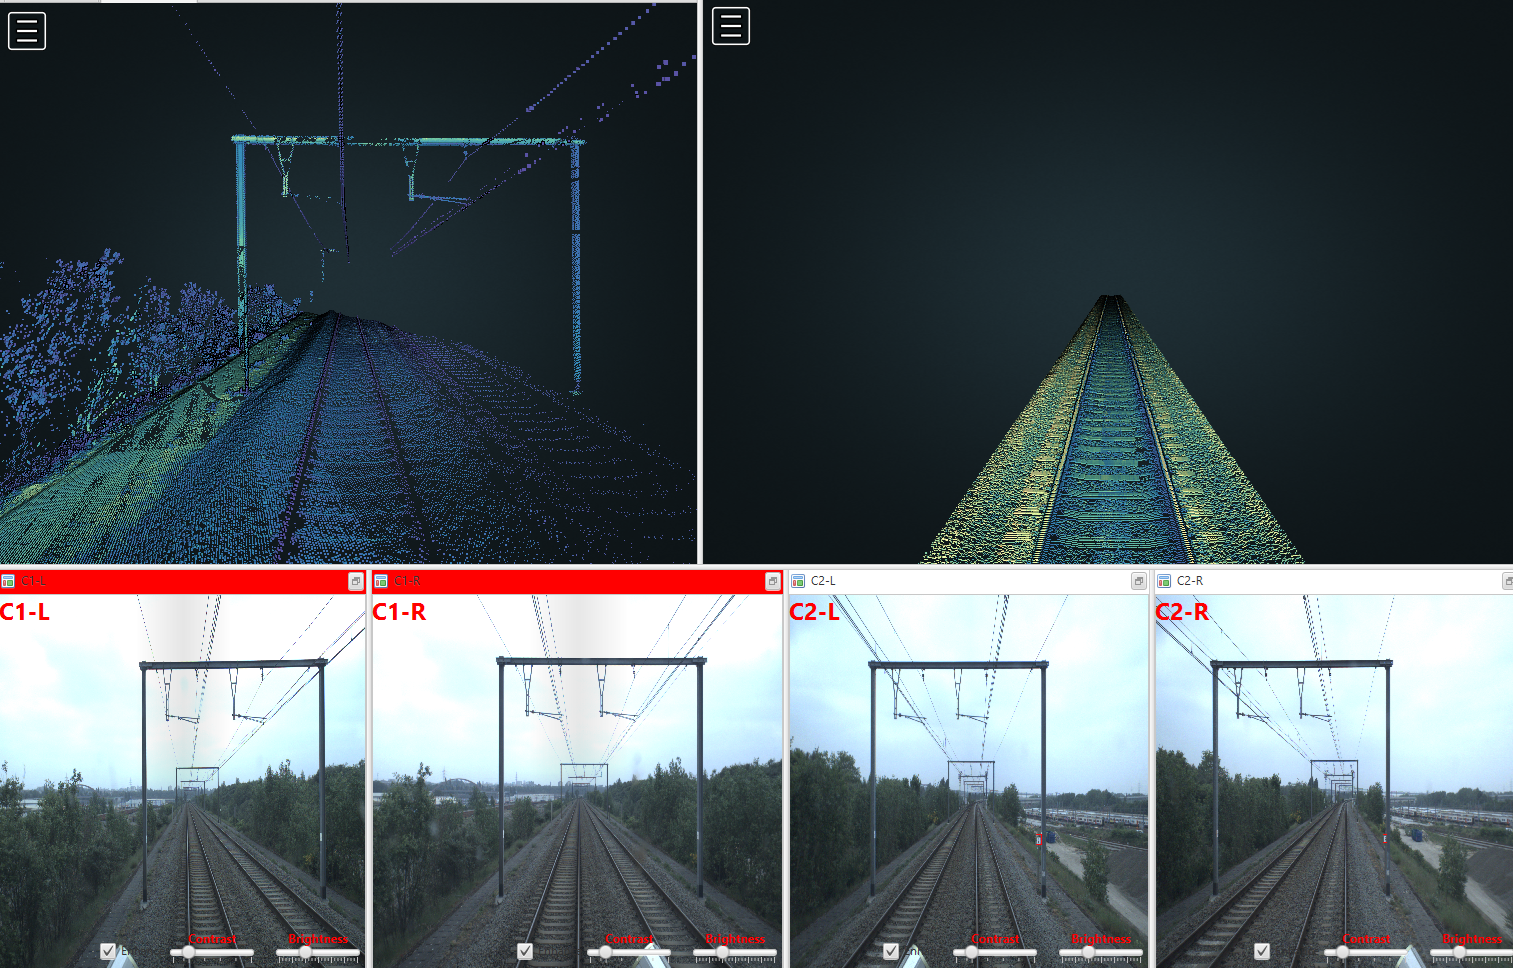
\includegraphics[width=12cm]{images/Hyperion-Interface.png}}   
            \caption{Visualisation dans Hyperion des nuages de points et des images relevés au cours d'une \gls{campagne}.} 
        \end{figure}
    \item 
Un système de reconnaissance et de vérification de la présence des éléments d'infrastructure a été développé à Bruxelles par ADCIS. Ce système consiste à synchroniser les données recueillies par tous les capteurs pendant une campagne, à géolocaliser ces données, à détecter et identifier les éléments ferroviaires, puis à les comparer avec des mesures antérieures (\textit{cf.} Figure 3). 
    
     \begin{figure}[H]
        \centering
        \fbox{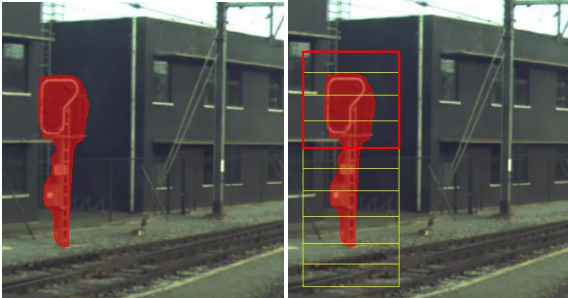
\includegraphics[width=10cm]{images/Hyperion-Identification.png} }  
        \caption{Identification et détection d'un élement ferroviaire - Documentation Cegelec \cite{Hyperion-interface}} 
    \end{figure}   
    
\end{itemize}


\subsection{Objectifs} 

L'objectif du projet est la conception d'un système informatique déstiné à analyser les données collectées par les trains de mesure d'Infrabel (\textit{cf.} Section 1.2), afin de développer un outil de maintenance prédictive du ballast férroviaire (\textit{cf.} Section 2), en se basant sur les paramètres fonctionnels tels que ceux qui suivent.

\begin{itemize}
\item \textbf{La vitesse} du train qui indique la direction de déplacement, soit vers l'avant (positif), soit en marche arrière (négatif). En cas de changement de direction d'un train, un nouveau segment est créé pour éviter la répétition d'une même portion de voie dans un seul segment.

\item \textbf{Le réseau}, qu'il soit un réseau conventionnel ou dédié aux lignes à grande vitesse.

\item \textbf{La structure}, c'est-à-dire les éléments physiques situés à gauche, à droite ou des deux côtés tels qu'un mur, un quai de gare, un pilier en béton, etc.

\item \textbf{La topologie}, il s'agit de la configuration de la proximité d'autres voies dans l'environnement, que ce soit simple ou double.

\item \textbf{La courbe} désigne la forme de la voie, pouvant être droite, courbée ou inclinée.

\item \textbf{Les zones exclues}, ce sont des zones où l'analyse du ballast ne doit pas être réalisée, telles que les ponts, les tunnels, les passages à niveau, les interrupteurs simples, les interrupteurs doubles et les interrupteurs de croisement.

\item \textbf{Les composants de voie} tels que le \gls{crocodile}, l'\gls{ETCS}.

\item \textbf{Les traverses} sont de différents types et peuvent être observés sur le terrain. Elles sont fabriquées en bois ou en acier (WS), ou encore en béton avec différentes formes, telles que les monoblocs (MB3, MB5, etc.) ou les biblocs (BB1, BB2, etc.). \cite{RHEA}
\end{itemize}


\noindent Les paramètres fonctionnels jouent un rôle essentiel dans l'établissement du profil théorique du ballast. Ce profil théorique sert de référence lors de la comparaison avec les données relevées, permettant ainsi de détecter d'éventuels déficits ou excès de ballast.\\

\noindent L'objectif du stage, quant à lui, peut être articulé sur trois points distintcs. 

\begin{itemize}
    \item \textbf{Identification du Type de Traverse de Voie} \\
    Le système vise à mettre en place une technologie permettant l'identification précise du type de traverse. Ces traverses peuvent être en bois, en métal ou en béton, possédant chacune un ensemble de sous-types spécifiques.
    
    \item \textbf{Identification de voies adjacentes à la voie courante} \\
    L'identification de la topologie de la voie est importante, car l'absence de voie à proximité se traduit par la formation d'un épaulement aux extremités du profil de référence, tandis que la présence d'une voie se caractèrise par un profil plat. Les configurations de topologies suivantes doivent être identifiées : simple voie, entre voie - voie à gauche, entrevoie - voie à droite, entrevoie - voies à gauche et droite. 

    \item \textbf{Localisation de la végétation} \\
    En complément, le système pourrait intégrer une fonctionnalité de détection de la végétation pour compenser le volume supplémentaire généré par la forme de la végétation lors de l'analyse du ballast. Cette fonctionnalité serait également utilisée afin d'optimiser la gestion de la végétation le long des voies ferroviaires. Actuellement, l'identification des zones nécessitant un entretien de la végétation se fait par relevé pédestre. L'objectif est de mettre en place un processus automatisé capable de cartographier les endroits présentant de la végétation nécessitant un entretien.

\end{itemize}





% parler que selon le type de ballast on veut derterminer le type de traverse qu'on devrait mettre. Les traverses sont de différents types et ils sont poser selon différents critères, il serait judicieux de les connaitre. 

%Lidar : 
%Est une caméra qui permet 
% parler ici de balast de voie, de lidar, de stéréovision, Odomètre, de naviagetion inertielle. Enfin tout ce qui permettra de comprendre le projet. 








































\section{RHEA}
Infrabel, en partenariat avec Cegelec Infra Technics et ADCIS, utilise des trains de mesure afin de vérifier les données topographiques du réseau férroviaire (\textit{cf.} Section 1.2). L'objectif d'Infrabel est d'exploiter ces données à d'autres fins, notamment l'évaluation de la quantité de ballast, en identifiant les zones présentant un excès ou un manque de ballast. Cette analyse vise à faciliter la maintenance prédictive en générant une cartographie colorée signalant les zones nécessitant une intervention. Cette approche simplifie la planification des campagnes d'entretien, actuellement basée sur des relevés pédestres. Cette section se concentre sur la présentation du projet inspirée de la documentation fournie par Cegelec \cite{RHEA}. 

\subsection{Présentation}
Infrabel envisage de mettre en place le projet RHEA pour analyser la pose du ballast, une composante importante du réseau ferrroviaire, qui soutient les rails et distribue au sol les contraintes mécaniques générées par le passage des trains. L'objectif principal de ce projet est de développer un système informatique capable de repérer les différents paramètres fonctionnels (\textit{cf.} Section 1.3) qui influencent la pose du ballast le long des voies ferroviaires.\\

Cette démarche vise à évaluer la concordance entre la pose théorique du ballast, enregistrée dans un registre chez Infrabel, et sa pose réelle obtenue grâce aux données collectées par Hyperion. L'analyse permettra de détecter d'éventuels surplus ou manques de ballast. Le résultat de cette évaluation sera utilisé pour générer une carte colorisée, facilitant ainsi la mise en oeuvre d'une maintenance prédictive ciblée. \\

L'analyse du ballast le long des rails repose sur les données fournies par plusieurs capteurs d'Hyperion ainsi que sur les données résultant de la phase de compilation. Parmi celles-ci, on peut citer :
\begin{itemize}
    \item \textbf{Les capteurs lidar 2D} \\

    
      Un Lidar 2D est un capteur équipé d'un laser et d'un élement récepteur, tel qu'une caméra (\textit{cf} Figure 4.a), permettant d'émettre un point laser sur une surface à mesurer. La lumière réfléchie par la surface atteint ensuite la caméra sous un angle particulier, ce qui permet de calculer la distance qui sépare la surface du capteur (\textit{cf} Figure 4.b \cite{triangulation}). Les distances mesurées produisent une représentation en deux dimensions de l'environnement. \\

    \begin{figure}[H]
      \centering
      \fbox{\subcaptionbox{}{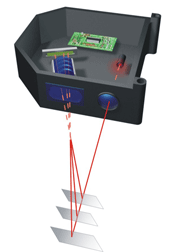
\includegraphics[width=2.35cm]{images/Lidar2D.png}}}
      \qquad % Add some space between the two subfigures
      \fbox{\subcaptionbox{}{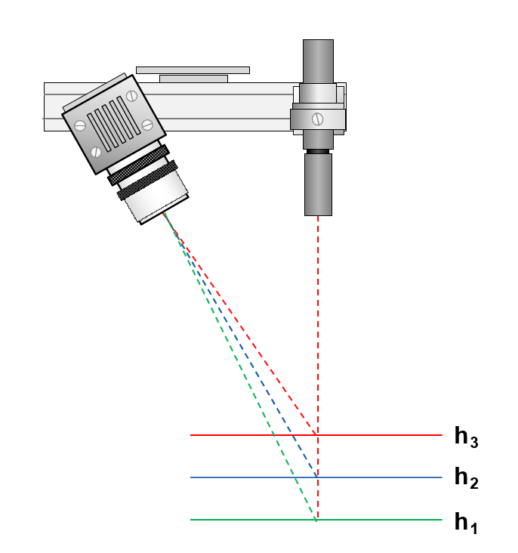
\includegraphics[width=3cm]{images/laser_triangulation.png}}}
      
      \caption{Lidar 2D}
    \end{figure}

    Quatre capteurs ont été fixés sous le plancher des trains de mesure, comme illustré sur la Figure 5,  pour recueillir les profils du sol le long d'une ligne d'observation de 4 mètres, avec une mesure effectuée tous les 4 centimètres, indépendament de la vitesse du train. L'ordonnée de ce système est centrée entre les 2 capteurs intérieurs en x et alignée sur ces deux derniers en y.


    \begin{figure}[H]
            \centering
           \fbox{ 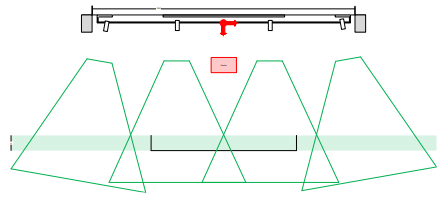
\includegraphics[width=6cm]{images/2dLidarmechaniacalimprementation.png}    }
            \caption{Méchanique d'implémentation du Lidar 2D - Cegelec \cite{RHEA}} 
        \end{figure}
    
    
    \item \textbf{Le Système de navigation inertielle} \\
    
    Le système de navigation inertielle adopté pour les trains de mesure repose sur l'Atlans-C (\textit{cf}. Figure 6). Ce système, tel que décrit par IXBlue dans sa documentation \cite{Atlans-c}, inclut un ensemble de composants comprenant un système de positionnement par satellites ou Global Navigation Satellite Systems en anglais (\gls{GNSS}), un gyroscope à fibre optique, un accéléromètre, ainsi qu'un récepteur GNSS \gls{RTK} pour des corrections en temps réel visant à atteindre une précision de l'ordre du centimètre. Cette configuration assure une détermination précise de la position, de la vitesse, de l'accélération, et de l'orientation du train, même dans des conditions complexes telles que les passages à travers des tunnels.

    \begin{figure}[H]
            \centering
           \fbox{ 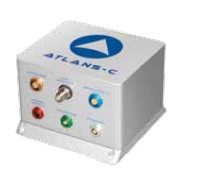
\includegraphics[width=4cm]{images/atlans-c.png}   
           }
            \caption{INS - Atlans-C \cite{Atlans-c}} 
        \end{figure}

    
    \item \textbf{La liste des éléments au sol}  \\
    
   Les profils obtenus lors de la campagne de mesure sont combinés et géolocalisés. Une image virtuelle, comme présentée dans la Figure 7, est générée à partir de ces profils, puis soumise à une intelligence artificielle chargée de repérer et d'identifier les éléments au sol, tels que les passages à niveau, les aiguillages simples ou doubles, les crocodiles, etc. Une liste exhaustive de ces éléments est ensuite produite à la fin du processus de compilation. 

    \begin{figure}[H]
            \centering
           \fbox{ 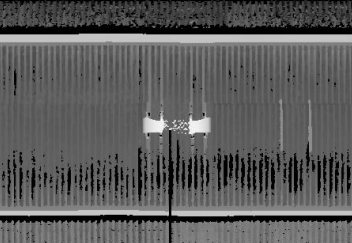
\includegraphics[width=5cm]{images/ground_list.png}   
           }
            \caption{Image virtuelle 2D - Cegelec \cite{RHEA}} 
        \end{figure}
    
\end{itemize}







\subsection{Fonctionnement}

Infrabel dispose dans ses registres d'un standard de pose du ballast qui repose sur plusieurs paramètres fonctionnels, comme introduit dans la Section 1.3 de notre étude. L'identification de ces paramètres fonctionnels permet d'établir le profil théorique du ballast, ensuite comparé avec le profil relevé, comme illustré dans la Figure 8.


\begin{figure}[H]
            \centering
           \fbox{ 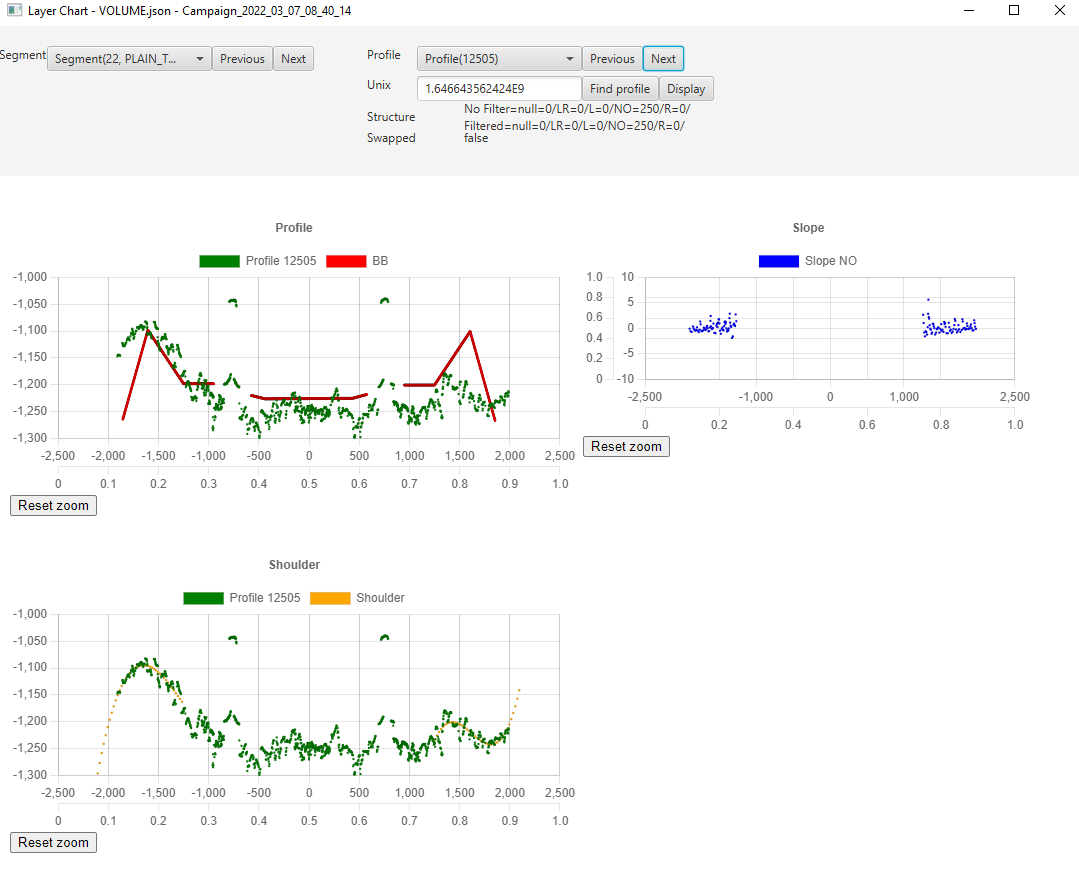
\includegraphics[width=10cm]{images/ballast-fx.PNG}   
           }
            \caption{Interface - Ballast FX } 
        \end{figure}

Cette représentation, générée à l'aide de Ballast FX, une interface créée en JavaScript dédiée à la comparaison des profils, met en évidence en rouge le profil théorique, tandis qu'en vert, un point de nuage représente le ballast réel. Cette visualisation permet d'identifier d'éventuelles variations, signalées par des zones où le ballast diffère du profil théorique. Les points verts situés au-delà de la ligne rouge pourraient signaler un excès de ballast, tandis que des zones sans points pourraient révéler un manque de ballast. \\

    \begin{figure}[H]
            \centering

           \fbox{ 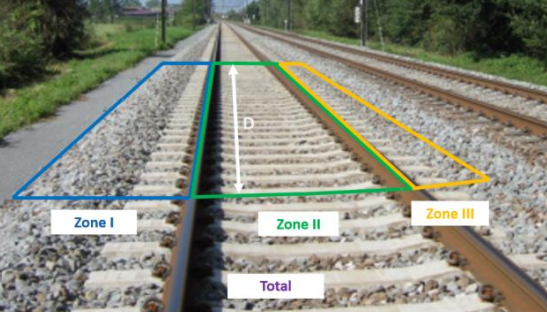
\includegraphics[width=8cm]{images/zones.png}   
           }
            \caption{Zone 1, 2 et 3 - Cegelec \cite{RHEA}} 
        \end{figure}
    


L'analyse du ballast est réalisé sur des segments de voie, qui représentent de petites fractions de la voie présentant des caractéristiques communes sur toute leur longueur. Cette analyse repose sur trois zones distinctes (\textit{cf.} Figure 9) pour identifier le manquement ou les excès de ballast. Ces zones sont : 


\begin{itemize}
    \item Zone 1 correspond à la partie gauche du rail gauche ;
    \item Zone 2 se situe entre les rails ;
    \item Zone 3 concerne la partie droite du rail droit.
\end{itemize}

\noindent Une fois cette analyse effectuée, les zones requérant une intervention sont enregistrées dans un fichier JSON au format GeoJSON. Ce fichier peut ensuite être intégré dans un système d'information géographique, tel que le logiciel QGIS (Quantum Geographic Information System), afin de générer une cartographie où les zones nécessitant une intervention sont visualisées en couleur, comme démontré dans la Figure 10.\\
\begin{figure}[H]
            \centering
           \fbox{ 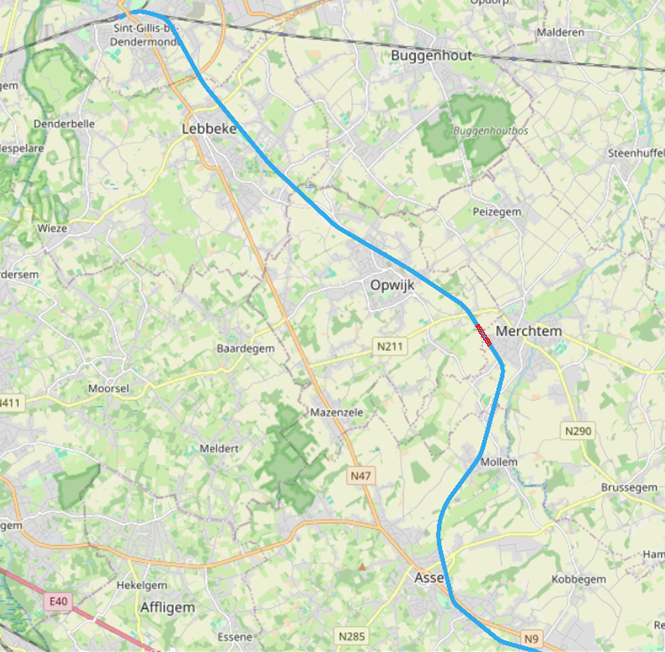
\includegraphics[width=6cm]{images/QGIS.PNG}   
           }
            \caption{Cartographie des zones nécessitant une intervention - QGIS } 
        \end{figure}

Cette cartographie offre une visualisation claire des zones spécifiques où des ajustements sont nécessaires, facilitant ainsi la planification des travaux de maintenance et contribuant à la gestion de la qualité du ballast sur le réseau ferroviaire.


\subsection{Définition du problème}


Pour effectuer l'analyse du ballast, l'accès aux données collectées au cours d'une campagne de mesure est essentielle. Ces données, stockées dans un fichier appelé *.campaign, peuvent être récupérées à l'aide des web services intégrés dans le code Java. Elles sont indispensables pour comparer la pose réelles et la pose théorique du ballast.\\
\newpage

\noindent La forme théorique du ballast est déterminée en fonction de divers paramètres fonctionnels (\textit{cf.} Figure 11). Il est impératif d'identifier ces paramètres pour sélectionner la forme théorique adéquate et conduire ainsi une analyse du ballast.\\

\begin{figure}[H]
            \centering
           \fbox{ 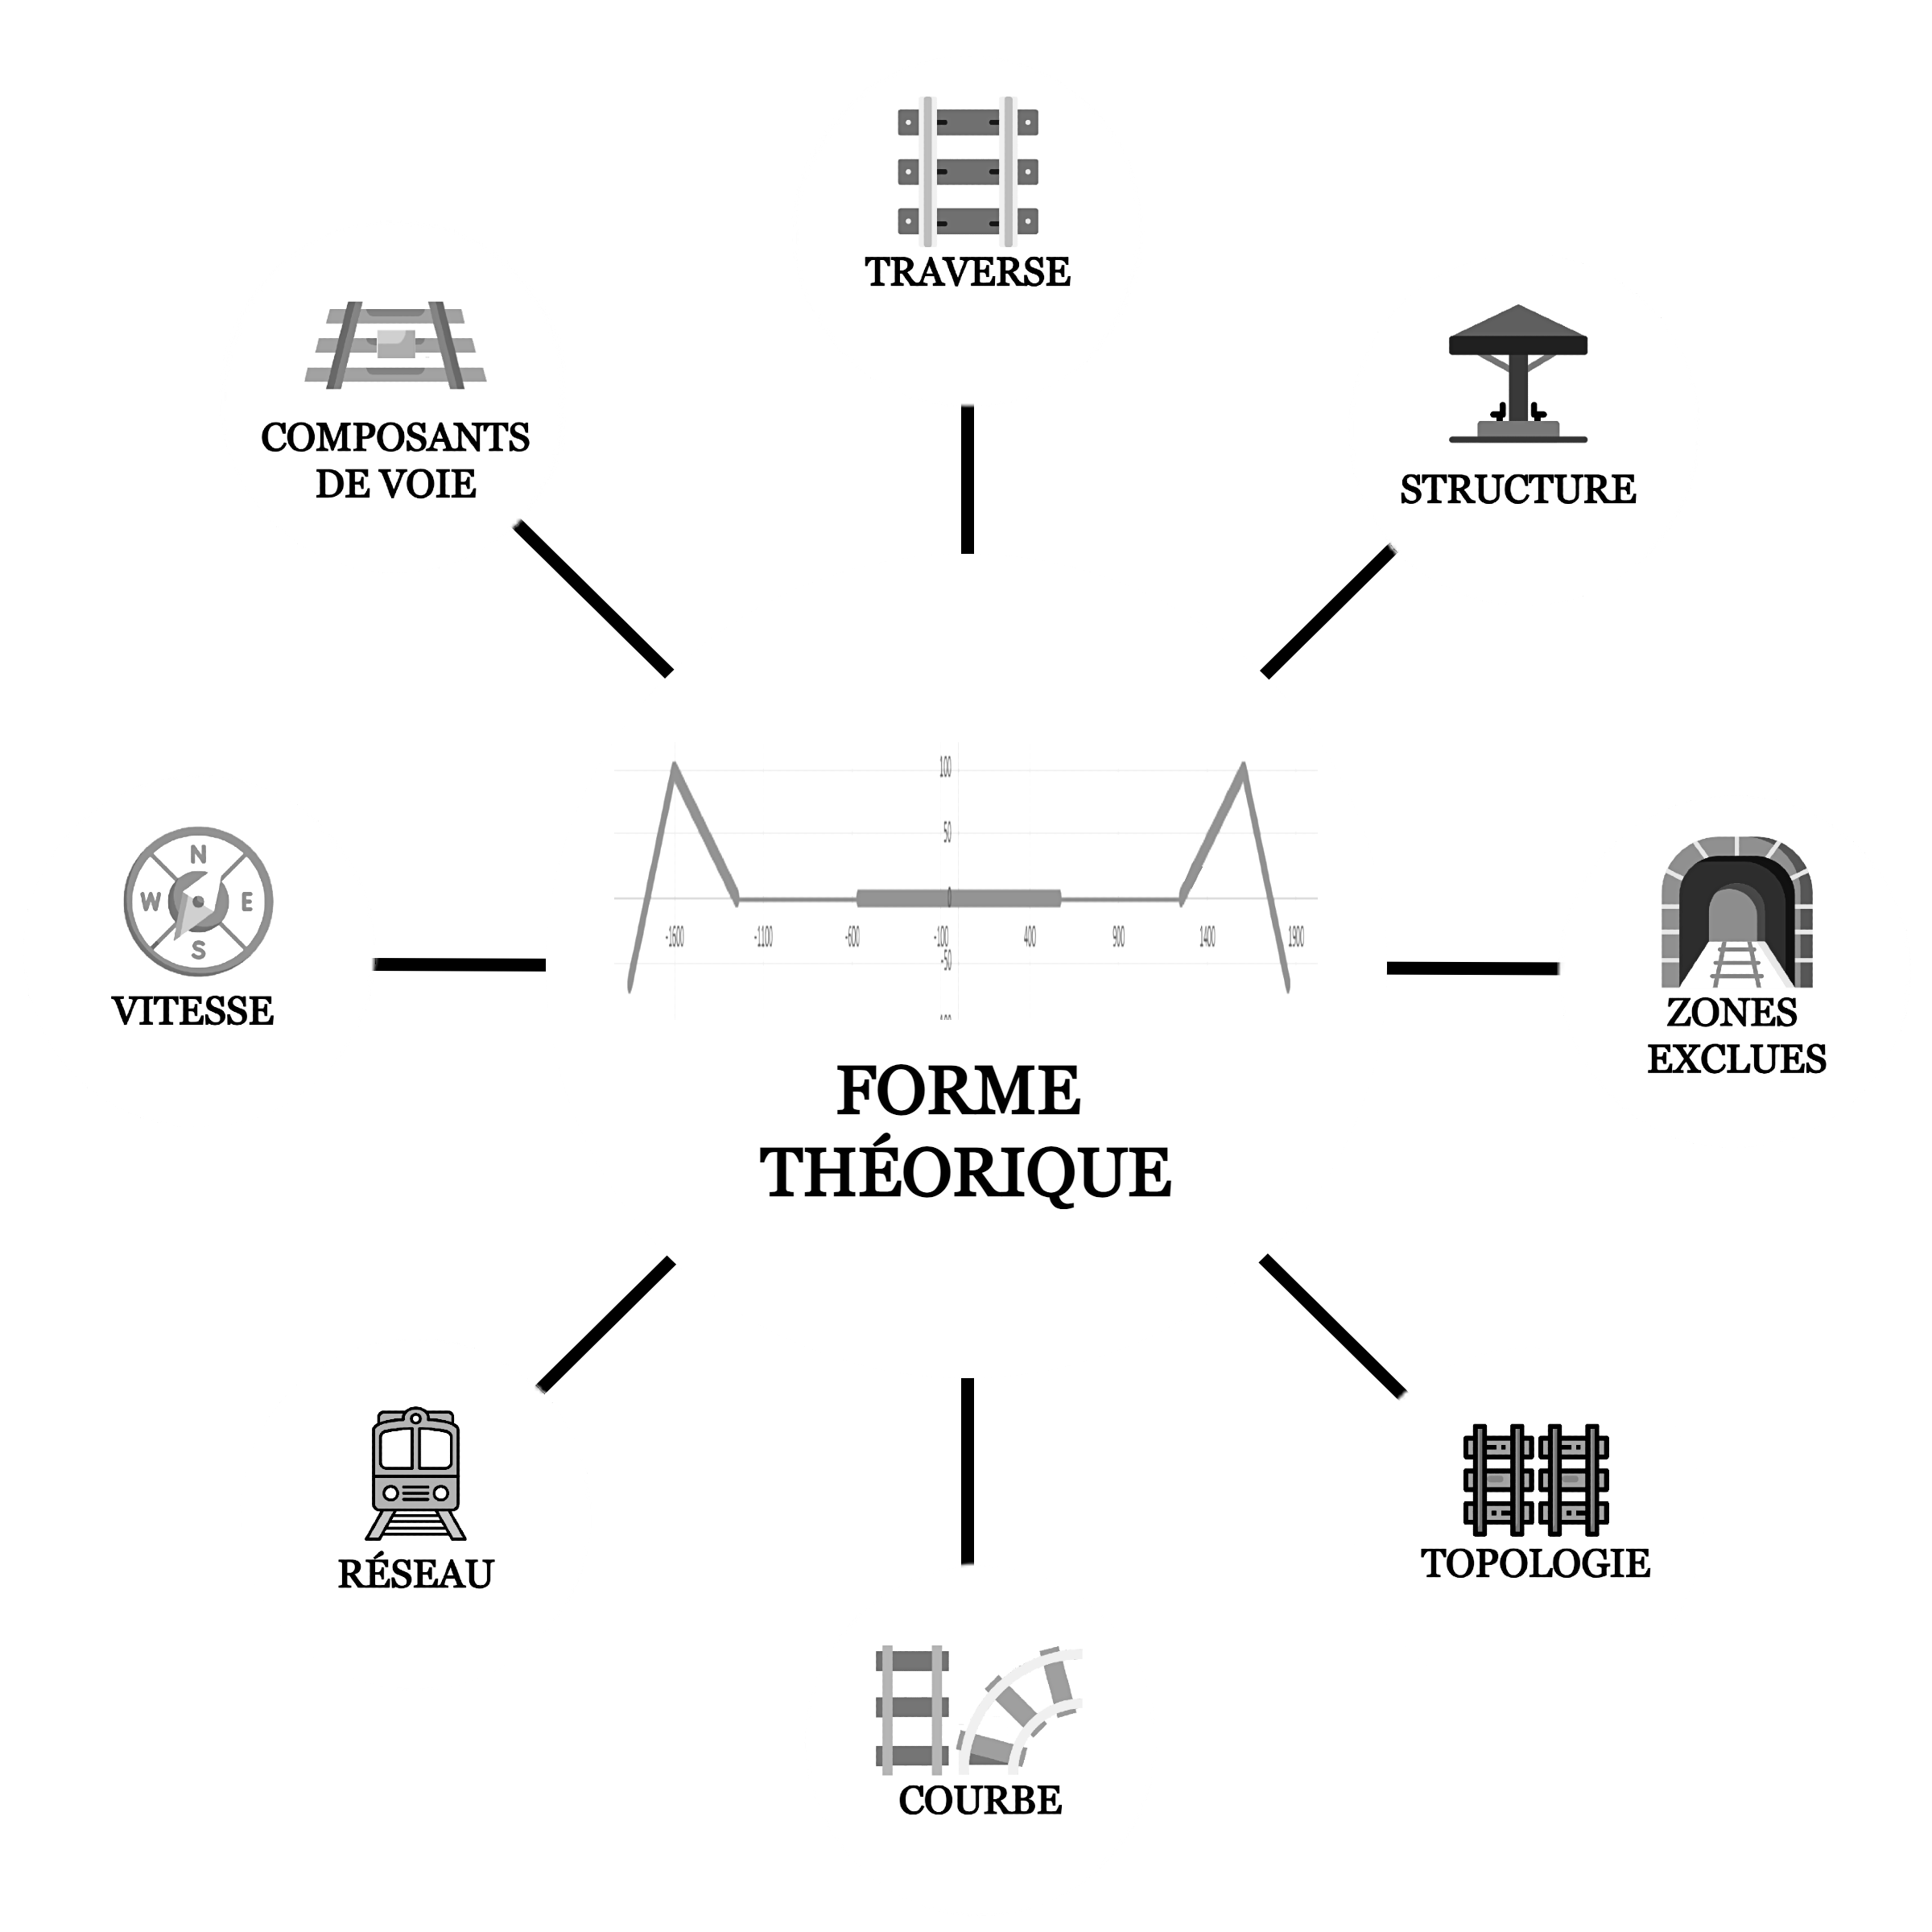
\includegraphics[width=7cm]{images/PARAMFONC1.png}   
           }
            \caption{Paramètres fonctionels } 
        \end{figure}


\noindent Certains paramètres, tels que la vitesse, le type de réseau, la structure, les zones exclues et les composantes de voies, sont déjà identifiés et constituent une base de données essentielle pour l'analyse. \\


\noindent Cependant, d'autres paramètres tels que le type de traverse et la topologie nécessitent une étude approfondie, et ces éléments constituent les objectifs principaux de ce stage, comme précisé dans la Section 1.3. \\


\noindent En ce qui concerne le type de traverse, une première approche de détection repose sur une méthode mathématique qui fonctionne de manière raisonnable, c'est-à-dire qui identfie correctement les traverses. Toutefois, certaines limitations se manifestent dans des conditions spécifiques. Les détails de cette approche, ainsi que ses limitations, sont couverts dans la Section 4. Pour remédier à ces limitations, la Section 5 présente une analyse basée sur des modèles d'intelligence artificielle. Cette analyse permet de comparer les deux approches afin de déterminer la plus performante  pour la détection du type de traverse. \\

 \noindent La détection de la topologie repose aussi sur une approche d'IA et elle sera étudié ultérieurement si le temps le permet. 
% montrer une exemple de la carte cartographié, d'une comparaison entre le ballast et le profil théorique. parler des différents paramètre fonctionnelles qui doivent être derterminer au préalable. Dire par exemple que la traverse est en cours d'études car c'est la cas de mon stage que la vitesse on l'obtient directement, parler de la topologie de la voie, les grounds element on a déjà donc çava comme le ETCS ou le simple track. Parler qu'on doit identifier si il y a des voies à proximité des voies adjacentes. 


% Parler de comment les enregistrement sont fait, tous les 4 centimètres etc
% COmment l'analyse du profil se fait 

% Parler des données récolter, quelles sont ses données sous quelles formes sont-elles ? 


\subsection{Objectif}
L'objectif principal du projet, comme énoncé dans la Section 1.3, est d'assurer une identification précise des paramètres fonctionnels liés à la pose du ballast, tels que le type de traverse ou la topologie, afin de mettre en place un système de maintenance prédictive pour les voies ferrées. Ceci sera réalisé en se basant sur l'analyse des données collectées par des capteurs au niveau du sol. \\

Le projet sera divisé en trois parties, chacune représentant un aspect distinct des objectifs du stage, et suivra le schéma suivant.
\begin{enumerate}
    \item Collecte des données : La première étape du projet consiste à collecter les données en examinant leur format et leur disposition, afin d'extraire celles qui seront utiles pour l'analyse du ballast.

    \item Exploration des données et développement de modèles d'IA : Ensuite, les données seront explorées en utilisant différentes méthodes d'IA pour identifier les profils des traverses ferroviaires. Cela impliquera de définir une stratégie de détection et de choisir les modèles de classification appropriés.
\newpage
    \item Évaluation et intégration : Après avoir examiné ces méthodes, nous évaluerons la précision des modèles afin d'atteindre les objectifs d'identification les plus précis possible. Ensuite, nous étudierons les possibilités d'intégrer les outils d'IA développés en Python dans l'écosystème Java, en explorant diverses approches telles que l'utilisation d'API, de scripts ou d'autres méthodes pour déterminer la meilleure méthode d'intégration.
\end{enumerate}




\section{Introduction à l'Intelligence Artificielle (IA)}

Cette section se base sur la documentation fournie par DataCamp \cite{datacamp} et explore le vaste domaine de l'intelligence artificielle. L'intelligence artificielle est un domaine vaste qui vise à permettre aux machines d'imiter le comportement humain. Il comprend plusieurs branches, dont l'apprentissage automatique, qui permet à une machine ou un système d'apprendre ou de s'améliorer sans ou avec très peu d'intervention humaine. On distingue généralement trois approches de l'apprentissage automatique : l'apprentissage supervisé, l'apprentissage non supervisé et l'apprentissage par renforcement. \\

\noindent Dans l'apprentissage supervisé, un modèle est entraîné à partir d'un ensemble de données étiquetées, tandis que dans l'apprentissage non supervisé, le modèle doit découvrir par lui-même des structures ou des relations dans des données non étiquetées. Dans l'apprentissage par renforcement, le modèle reçoit des récompenses ou des pénalités en fonction des décisions qu'il prend. \\


\noindent Pour notre étude, nous allons nous focaliser sur une sous-branche de l'apprentissage automatique, connue sous le nom d'apprentissage profond et plus précisement l'apprentissage par réseau de neurones. Cette approche permet aux systèmes informatiques d'imiter la structure et le fonctionnement des neurones humains, grâce à des réseaux de neurones artificiels. L'apprentissage profond est largement utilisé pour la classification et offre des capacités puissantes en matière de modélisation et de représentation des données complexes.

\subsection{Choix de la méthode d'IA}

L'apprentissage profond, comme mentionné précédemment, reproduit la structure et le fonctionnement des neurones humains à travers des neurones artificiels, afin de découvrir des relations complexes entre les données. En effet, les neurones biologiques sont constitués de dendrites et d'axones, qui reçoivent et émettent des signaux, correspondant respectivement à l'entrée et à la sortie du neurone. Ces concepts sont modélisés par des entrées et des sorties dans les modèles de neurones artificiels. La Figure 13 présente une comparaison entre un neurone biologique et la forme la plus simple d'un réseau de neurones, le perceptron. \\

\begin{figure}[H]
            \centering
           \fbox{ 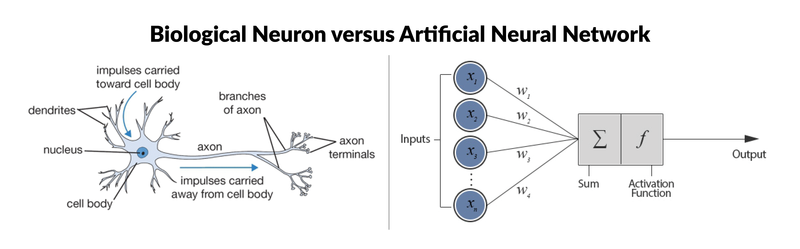
\includegraphics[width=15cm]{images/content_content_neuron.png}}   
            \caption{Comparaison d'un nerone avec un perceptron  -  \cite{datacamp}} 
        \end{figure}

\noindent Un perceptron peut être considéré comme une fonction mathématique qui prend en entrée un ensemble de données, effectue des opérations spécifiques, applique une fonction d'activation pour réguler les valeurs dans un intervalle selon la fonction choisie, et produit ensuite un résultat en sortie. \\

\begin{equation}
\hat{y} = \sigma(\sum_{x \in X } x \theta )
\label{moneq}
\end{equation} 
\vspace{1cm}

\noindent L'équation \eqref{moneq} entraîne plusieurs éléments, chacun ayant un rôle spécifique. La notation $\sum_{x \in X} x \theta$ représente la somme pondérée des entrées, où $x$ correspond aux différentes valeurs des caractéristiques de l'entrée, $\theta$ désigne les poids et biais associés à ces caractéristiques, et la sommation est effectuée sur l'ensemble des caractéristiques de l'entrée $X$. La fonction d'activation $\sigma$ est appliquée à la somme pondérée des entrées pour produire $\hat{y}$, qui représente la prédiction du modèle. \\

\noindent Les modèles basés sur un simple perceptron fonctionnent en classifiant les données en seulement deux classes à l'aide d'une limite tracée par une ligne droite, ce qui n'est pas adapté lorsque plusieurs classes sont présentes. Pour surmonter cette limitation, des modèles plus complexes existes. Elles sont constitués de différentes couches contenant un ensemble de perceptrons qui interagissent entre-eux pour extraire les caractéristiques essentielles des données en vue de leurs classifications. (\textit{cf.} Figure 13).\\


\begin{figure}[H]
            \centering
           \fbox{ 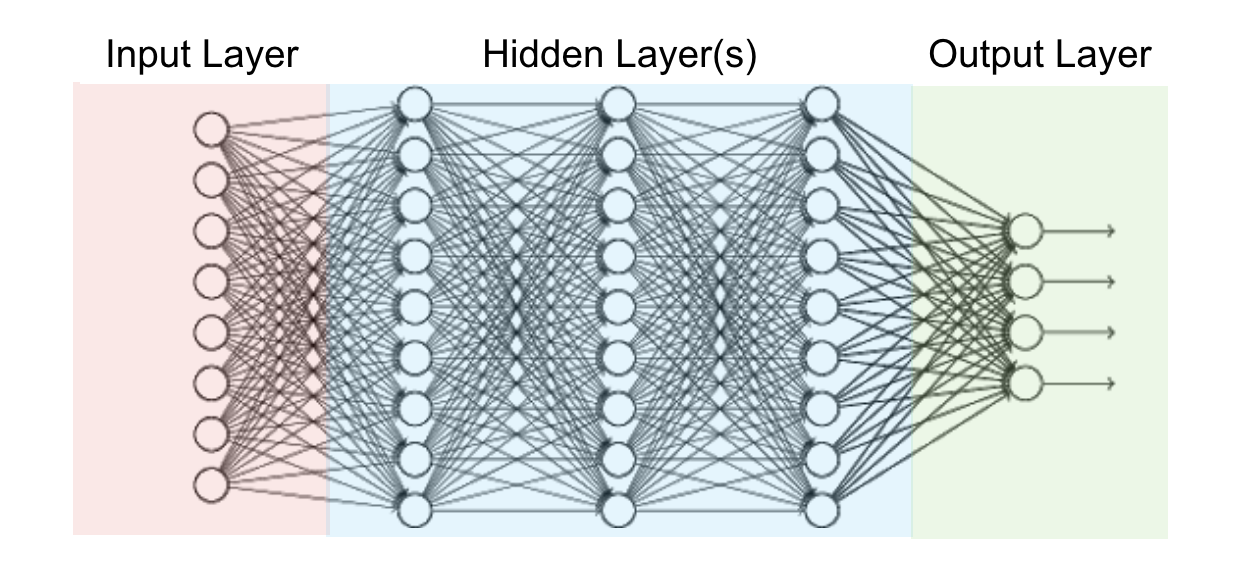
\includegraphics[width=12cm]{images/HiddenLayers.png}}   
            \caption{Illustration des diverses couches dans l'apprentissage profond -  \cite{hiddenlayer}} 
        \end{figure}


\noindent L'entraînement de nos données se déroulera sur des réseaux de convolution, exploitant la rétropropagation du gradient. Cette technique permet de mettre à jour les paramètres $\theta$ du modèle, afin de minimiser la fonction de coût.\\


\noindent La fonction de coût est généralement calculée comme la moyenne des fonctions de perte pour chaque exemple de données. Ces fonctions de perte mesurent la différence entre les valeurs réelles et les valeurs prédites par le modèle. En minimisant cette fonction de coût, l'objectif est d'améliorer les performances globales du modèle en termes de précision et de capacité de généralisation.\\

\noindent Cette approche permet aux réseaux de neurones profonds de capturer des caractéristiques complexes dans les données, ce qui les rend efficaces pour la classification et l'identification de données.



\subsection{Environnement de travail}

Cette section est inspirée des consignes fournies par le site de TensorFlow \cite{TensorFlow} pour configurer un environnement de travail afin d'exploiter pleinement la capacité du GPU et d'optimiser l'utilisation des modèles d'apprentissage profond. Étant donné que la dernière version de TensorFlow prenant en charge le GPU sur Windows natif est la version 2.10, nous avons choisi de configurer la version 2 du Windows Subsystem Linux qui permet de lancer des exécutables Linux sur Windows. Cette solution permet de profiter des versions plus récentes de TensorFlow. \\

\noindent De plus, nous avons configuré Visual Studio Code pour qu'il fonctionne correctement avec TensorFlow en utilisant le GPU. Nous avons ainsi suivi les étapes suivantes. \\

\begin{itemize}
    \item Nous avons installé et configuré Windows Subsystem for Linux version 2 (WSL2) sur mon système.
    \item Nous avons ensuite procédé à l'installation et à la configuration d'Ubuntu dans WSL2, créant ainsi un environnement Linux fonctionnel ;
    \item Nous avons installé la dernière version de TensorFlow compatible avec l'utilisation du GPU, afin de bénéficier de ses performances optimales ;
    \item Pour permettre à TensorFlow d'utiliser le GPU, Nous avons  installé les pilotes NVIDIA nécessaires pour CUDA.
Nous avons configuré Visual Studio Code pour exécuter le code dans le nouvel environnement Linux, assurant ainsi une intégration fluide avec mes projets TensorFlow ;
    \item Enfin, Nous avons vérifié que le GPU était correctement configuré et utilisé par TensorFlow, ce qui nous a permis d'exécuter nos codes et nos modèles sur le GPU avec succès.
\end{itemize}

\subsection{Conclusion}

En conclusion, l'intégration de l'intelligence artificielle, notamment à travers l'apprentissage profond et la configuration de l'environnement de travail avec TensorFlow sur un GPU, sont bénéfique pour traiter les données complexes obtenues des capteurs d'Hyperion. Les réseaux de neurones sont capables d'analyser les relations complexes de ces données et d'extraire des informations cruciales pour les identifier, même lorsque celles-ci ne sont pas visibles à premiere vue. D'autre part, la configuration du GPU accélère le processus d'apprentissage des modèles, permettant ainsi d'économiser du temps. Ensembles, ces technologies permettent d'identifier les traverses et la topologie de façon plus précise et rapide.




\section{Besoins et contraintes du projet}

Dans cette section, nous exposons les éléments essentiels du projet, détaillant les besoins et contraintes nécessaires à sa réussite.


\subsection{Besoins}
Avant de se lancer dans un projet, il est crucial d'identifier les besoins essentiels qui détermineront sa réussite. Ces besoins servent de guide et permettent à atteindre les résultats souhaités à la fin du projet. Cette sous-section les présente. \\

\noindent \textbf{Précision de l'identification} Le système doit garantir une identification précise des paramètres fonctionnels liés à la pose du ballast, tels que le type de traverse, la topologie de la voie, etc. \\

\noindent \textbf{Automatisation} \\
 La mise en place d'un processus automatisé est essentielle pour assurer l'efficacité opérationnelle, en particulier dans la détection des anomalies et la gestion de la végétation. \\
 
\noindent \textbf{Intégration de données} \\
Le système doit être capable d'intégrer et d'analyser les données recueillies par les trains de mesure d'Infrabel de manière cohérente et précise. \\

\noindent \textbf{Maintenance prédictive} \\
Le développement du système doit permettre la mise en place d'un outil de maintenance prédictive du ballast ferroviaire, en identifiant les zones nécessitant une intervention.
    


\subsection{Contraintes}
Cette sous-section présente, les contraintes et les défis à prendre en compte lors de la conception et la mise en oeuvre du projet. \\

\noindent \textbf{Contraintes technologiques} \\
L'intégration des modèles d'intelligence artificielle développés en Python peut présenter des défis majeurs en raison de l'écosystème principal utilisé en Java. L'absence de GPU dans le contexte Java peut affecter la performance et la compatibilité avec les modèles existants.\\

\noindent \textbf{Explicabilité des modèles} \\
 Certains modèles d'IA, en particulier les réseaux neuronaux complexes, peuvent être considérés comme des "boites noires". Dans le cas de ce projet, il est nécessaire de pouvoir comprendre et interpréter les résultats produits par les modèles d'apprentissage automatique.\\

\noindent \textbf{Complexité des variations du terrain} \\
Les petites variations, telles que la végétation cachant partiellement le ballast, présentent des défis pour l'identificaiton. \\

\noindent \textbf{Données limitées pour l'entraînement des modèles } \\
L'absence de données d'entraînement complètes pour tous les types de traverses peut limiter l'efficacité des modèles dans la reconnaissance et le traitement de certaines traverses. Cela souligne l'importance de mener des campagnes pour enregistrer tous les types de traverses.



\subsection{Conclusion}
En conclusion, le projet se déploie selon plusieurs étapes stratégiques. Nous commençons par l'identification du type de traverse en utilisant des modèles de classification simples, puis évoluons vers des modèles plus complexes. Une phase initiale de test se limite à une portion restrainte de données, par exemple deux types de traverses. Ensuite, nous utilisons le modèle pour inférer dans l'écosystème Java, en explorant des méthodes telles que l'utilisation d'API, de script, ou d'autres astuces. Enfin, nous évaluons le modèle pour garantir la précision attendue. Cette approche progressive vise à assurer le développment cohérent et efficace du projet. \\

\noindent Une fois cette première phase achevée, nous aurons l'opportunité d'examiner d'autres aspects du projet, notamment la détection des vois à proximité et la localisation de la végétation. 




% \subsection{Exigences Techniques}
% L'environnement de travail est constitué de logiciels tels que Python et Jupyter Notebook qui nous permettent d'analyser, de traiter et de présenter les données. nous utilisons également des librairies (\textit{cf.} Section 3.2) qui nous permettent de travailler de manière efficace sur des projets de data science et de répondre aux exigences techniques du domaine. 



\section{Identification du type de traverse de voie}

Cette section se concentre sur la présentation de la méthode existante, ainsi que sur l'exploration et l'analyse de nouveaux modèles afin de déterminer le type de traverse. Différentes modèles d'IA sont examinés afin de les évaluer et sélectionner le plus performant. 

\subsection{Exploration des Données}
% Dans un premier temps, la collecte des données se concentre sur trois types spécifiques de traverses, à savoir BB1, MB5 et WS. Ces données sont recueillies en fonction du type de segment identifié à l'aide de la méthode mathématique décrite dans la Section 5, et elles sont confirmées visuellement à travers l'interface Hyperion. Ces segment contiennent un certain nombre de profils par type. Le tableau X répertorie le nombre de profils par type qui seront utilisés lors d'une première approche.


%% Dire que j'ai eté sur hyperion pour prendre les données. Que j'ai checké chaque données à l'aide de QGIS puis j'ai vérifier si c'est vraiment ce type de traverse. J'ai aussi reagrder sur ballast FX pour comparer ce ballast si c'est bien ce type. 

Dans cette section, nous aborderons la récupération des données, leur traitement initial ainsi que l'application de techniques de data augmentation pour enrichir notre ensemble de données.
\input{B) Sections/Objectif_1/Modèle Existant}
\subsection{Approche 1}

Cette approche consiste à utiliser les données préparées dans la section 5.1  afin de développer un système de classification en utilisant un réseau de neurones convolutionnel (CNN) avec une convolution à une dimension. Dans cette approche, seuls les points sur l'axe vertical (y) de la traverse sont pris en compte pour l'analyse.


\subsubsection{Modèles et Analyse}
Cette section présente une gamme de modèles utilisés pour l'identification du type de traverses, accompagnée d'une analyse comparative visant à déterminer le meilleur modèle pour l'identification du type de traverses. \\

\subsection{Approche 2}
Cette approche consiste à utiliser à la fois les coordonnées horizontales (x) et verticales (y) des points de la traverse pour développer un système de classification. En intégrant ces deux dimensions, nous cherchons à obtenir une représentation plus complète des caractéristiques des traverses, ce qui pourrait améliorer la précision de notre modèle de classification par rapport à l'approche précédente.

\subsubsection{Modèles et Analyse}
Cette section présente une gamme de modèles utilisés pour l'identification du type de traverses, accompagnée d'une analyse comparative visant à déterminer le meilleur modèle pour l'identification du type de traverses. \\

\subsection{Approche 3}
Cette approche  consiste à utiliser les coordonnées horizontales (x) et verticales (y) des points de la traverse, ainsi que l'intensité des données. En intégrant ces trois dimensions, nous cherchons à obtenir une représentation encore plus complète des caractéristiques des traverses. Cela nous permettra d'explorer de manière plus approfondie les variations et les motifs présents dans les données, avec pour objectif d'améliorer la précision et la robustesse de notre système de classification.
\subsubsection{Modèles et Analyse}
Cette section présente une gamme de modèles utilisés pour l'identification du type de traverses, accompagnée d'une analyse comparative visant à déterminer le meilleur modèle pour l'identification du type de traverses. \\

%  \noindent Les modèles choisis seront entraînés à l'aide de la validation croisée sur des données d'entraînement composé de 2000 profils et évalués sur des données de test de 400 profils, afin de mesurer les performances de généralisation des modèles. \\

% \noindent En outre, chaque modèle sera évalué en utilisant différentes configurations d'hyperparamètres, comprenant des tailles de batchs de 8, 16, 32 et 64, ainsi que des taux d'apprentissage de 0.01, 0.001 et 0.0001. L'objectif est de sélectionner, pour chaque modèle, la configuration offrant les meilleures performances pour l'analyse comparative. \\

% \noindent L'analyse débutera avec des modèles simples pour ensuite être plus sophistiquées. \\

% \paragraph{Modèle 1} \\
% Ce modèle est composé de 3 couches et les résultats obtenues par les validation crosiées sont disponible dans les annexes avec la référence A. Ce modèle est composé de x paramètre entrainable et y paramètre non entrainable.
% \begin{figure}[H]
  \centering
  \begin{tikzpicture}
    \node[input,minimum width=2cm, minimum height=2cm] (x) at (-0.50,0)
    {\small Input};
 
    \node[conv,rotate=90,minimum width=4.5cm] (conv1) at (1.25,0) 
    {\small\textbf{Conv1D (32,2) + ReLU}};
    
    \node[flat,rotate=90,minimum width=4.5cm] (flat1) at (2.5,0) {\small\textbf{Flatten}};
    
    \node[dense,rotate=90,minimum width=4.5cm] (dense1) at (3.75,0) {\small\textbf{Dense (3) + Softmax}};

    \node[output,minimum width=2cm, minimum height=2cm] (y) at (5.5,0) 
    {\small\textbf{$Output$}};


    \draw[-] (x) -- (conv1);
    \draw[-] (conv1) -- (flat1);
    \draw[-] (flat1) -- (dense1);
    \draw[-] (dense1) -- (y);

  \end{tikzpicture}
  \vskip 6px
  \caption{An illustration of.}
\end{figure}

% \paragraph{Modèle 2}

% \input{D) Models/model2}

% \paragraph{Modèle 3}

% \begin{figure}[H]
  \centering
  \begin{tikzpicture}
    \node[input,minimum width=2cm, minimum height=2cm] (x) at (-0.50,0)
    {\small Input};
 
    \node[conv,rotate=90,minimum width=4.5cm] (conv1) at (1.25,0) 
    {\small\textbf{Conv1D (32,2) + ReLU}};
    
    \node[pool,rotate=90,minimum width=4.5cm] (pool1) at (2.5,0) {\small\textbf{MaxPooling1D (2)}};

    \node[drop,rotate=90,minimum width=4.5cm] (drop1) at (3.75,0) {\small\textbf{Dropout (0.5)}};

    \node[conv,rotate=90,minimum width=4.5cm] (conv2) at (5,0) 
    {\small\textbf{Conv1D (64,3) + ReLU}};

    \node[pool,rotate=90,minimum width=4.5cm] (pool2) at (6.25,0) {\small\textbf{MaxPooling1D (2)}};
    
    \node[flat,rotate=90,minimum width=4.5cm] (flat1) at (7.5,0) {\small\textbf{Flatten}};
    
    \node[dense,rotate=90,minimum width=4.5cm] (dense1) at (8.75,0) {\small\textbf{Dense (128) + ReLU}};
    
    \node[drop,rotate=90,minimum width=4.5cm] (drop2) at (10,0) {\small\textbf{Dropout (0.5)}};
    
    \node[dense,rotate=90,minimum width=4.5cm] (dense2) at (11.25,0) {\small\textbf{Dense (3) + Softmax}};

    \node[output,minimum width=2cm, minimum height=2cm] (y) at (13,0) 
    {\small\textbf{$Output$}};


    \draw[-] (x) -- (conv1);
    \draw[-] (conv1) -- (pool1);
    \draw[-] (pool1) -- (drop1);
    \draw[-] (drop1) -- (conv2);
    \draw[-] (conv2) -- (pool2);
    \draw[-] (pool2) -- (flat1);
    \draw[-] (flat1) -- (dense1);
    \draw[-] (dense1) -- (drop2);
    \draw[-] (drop2) -- (dense2);
    \draw[-] (dense2) -- (y);
  \end{tikzpicture}
  \vskip 6px
  \caption{An illustration of.}
\end{figure}





% Détaillez le processus d'intégration de l'IA dans le modèle existant.
% Expliquez comment les données sont utilisées, comment le modèle est formé, etc.
\subsection{Comparaison des Résultats}

% In this phase, a structure for a 1D-CNN model was proposed as a baseline. Then, to investigate the
% impact of different structures on the performance of the proposed model, another five CNN models
% with different structures in terms of dropout layer exclusion, kernel size, filter size, the inclusion of an
% additional convolutional layer, and type of convolutional and max pooling layers were constructed.
% After that, four machine learning models were developed to measure the efficiency of our proposed
% model compared to the established machine learning models.



%  In this paper, we aim to address such
% issues in predicting software defects. We propose a novel structure of 1-
% Dimensional Convolutional Neural Network (1D-CNN), a deep learning
% architecture to extract useful knowledge, identifying and modelling the knowledge in the data sequence, reduce overfitting, and finally, predict whether the
% units of code are defects prone. We design large-scale empirical studies to
% reveal the proposed model’s effectiveness by comparing four established traditional machine learning baseline models and four state-of-the-art baselines
% in software defect prediction based on the NASA datasets. The experimental
% results demonstrate that in terms of f-measure, an optimal and modest 1DCNN with a dropout layer outperforms baseline and state-of-the-art models
% by 66.79% and 23.88%, respectively, in ways that minimize overfitting and
% improving prediction performance for software defects. According to the
% results, 1D-CNN seems to be successful in predicting software defects and may
% be applied and adopted for a practical problem in software engineering. This,
% in turn, could lead to saving software development resources and producing
% more reliable software
\noindent Chaque modèle, avec sa configuration la plus performante, sera ensuite évalué en fonction des critères et pondérations. (Veille Technologique)
% Dire quelle fonction de cout on a utilsier. Et pourquoi. 

% Présentez la méthodologie de validation des résultats obtenus à partir du modèle mathématique et de l'IA.
% Comparez les performances des deux approches, en soulignant les avantages de l'utilisation de l'IA.
\subsection{Discussion sur les Avantages et les Limitations}

Discussion des avantages et limitations que l'intelligence artificielle apporte par rapport au modèle mathématique seul.
% Identifiez les limitations possibles de l'IA dans ce contexte.
\subsection{Perspectives Futures}
Suggestion des amélioration possibles.
% Suggérez des améliorations possibles de l'intégration de l'IA dans le modèle.
% Identifiez des domaines de recherche ou d'exploration potentiels.
% Conclusion de la Section :

% Résumez les principales contributions de l'utilisation de l'IA dans le contexte du modèle mathématique existant.
% Préparez la transition vers les sections suivantes de votre mémoire.
\subsection{Conclusion}
\section{Références}
\printglossary[title=Glossaire]
\renewcommand\refname{Bibliographie}
\begin{thebibliography}{9}

\bibitem{Hyperion-Unité}
ADCIS, Reconnaissance d'éléméents d'infrastructure ferroviaire. URL : https://www.adcis.net/fr/applications/hyperion-fr/ (Consulté le 21/12/2023)

\bibitem{Hyperion-interface}
Cegelec-IMCS, HYPERION - ARCHITECTURE AND DESIGN SPECIFICATION, Version 4, Bruxelles, 2017. 

\bibitem{triangulation}
MoviMED, What is laser Triangulation. URL : https://www.movimed.com/knowledgebase/what-is-laser-triangulation/, (Consulté le 28/12/2023)

\bibitem{RHEA}
Cegelec IMCS, RHEA - ARCHITECTURE AND DESIGN SPECIFICATION, Version 1, Bruxelles, 2023. 


\bibitem{Atlans-c}
IXBlue, Atlans-C, Mobile Mapping Position and Orientation Solution . URL : https://www.redimec.com.ar/contenido/productos/pdf/1433452247\_1.pdf (Consulté le 11/01/2024)

\bibitem{datacamp}
Karlijn Willems, Keras Tutorial, Deep Learning in Python. URL : https://www.datacamp.com/tutorial/deep-learning-python, 2019. (Consulté le 15/01/2024)

\bibitem{hiddenlayer}
Priyanshi SharmaPurpose of different layers in Deep , Learning Model. URL : https://iq.opengenus.org/purpose-of-different-layers-in-ml/, (Consulté le 15/01/2024)

\bibitem{TensorFlow}
TensorFlow, Installer TensorFlow avec pip.  https://www.tensorflow.org/install/pip?hl=fr#windows-native, 2023, (Consulté le 29/02/2024)

\end{thebibliography}

\end{document}